\documentclass{article}
% Language setting
% Replace `english' with e.g. `spanish' to change the document language
\usepackage[english]{babel}
% Set page size and margins
% Replace `letterpaper' with`a4paper' for UK/EU standard size
\usepackage[a4paper,top=2cm,bottom=2cm,left=3cm,right=3cm,marginparwidth=1.75cm]{geometry}

% Useful packages
\usepackage{amsmath}
\usepackage{graphicx}
\usepackage[colorlinks=true, allcolors=blue]{hyperref}

\title{Summary of Aortic Root Analysis}
\author{Ankush Aggarwal\thanks{A. Aggarwal is with the
Glasgow Computational Engineering Centre, James Watt School of Engineering, University of Glasgow, Glasgow, UK (e-mail:ankush.aggarwal@glasgow.ac.uk). }, Peter Mortensen, Jilei Hao, Paul Yushkevich, Alison M. Pouch \thanks{A. Pouch is with the Departments of Radiology and Bioengineering, University of Pennsylvania, Philadelphia, PA, USA (e-mail: pouch@pennmedicine.upenn.edu).}
%
\thanks{This work was supported in part by the Chan Zuckerberg Initiative 2020-219012 grant, the Institute of Physics and Engineering in Medicine, and the National Heart Lung and Blood Institute (K01-HL141643).}
}

\begin{document}
\maketitle
\begin{figure}[t!]

\includegraphics[width = 0.25\linewidth]{UPennLogo}~~~~~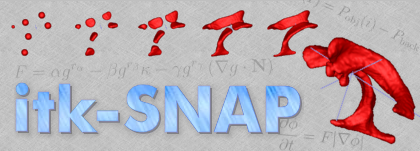
\includegraphics[width = 0.25\linewidth]{ITKSnapLogo}~~~~~
\includegraphics[width = 0.25\linewidth]{GlaLogo}~~~~~
\includegraphics[width = 0.1\linewidth]{GCEC}
\end{figure}
\newpage
\subsection*{Data Summary}
For each time frame in the 4D image, there are now .vtp/.vtk files. These files contain medial meshes of the root from the submitted image, with the applied labels and new biomechanical values that have been calculated. The data included are either specific to the points, to the cells, or are global data that are uniform over the whole field, as summarised next.
\\
~
\\
\begin{tabular}{|c|c|p{9.4cm}|}
	\hline
\textbf{Name}	& \textbf{Type} & \textbf{Description}   \\
	\hline
	\hline
	\multicolumn{3}{|c|}{\textbf{Anatomical Labels}} \\
	\hline
STJ	& Scalar  & Marks the sinotubular junction with value 1 and 0 elsewhere.  \\
	\hline
VAJ	& Scalar &  Marks the ventriculo-aortic junction with value 1 and 0 elsewhere.  \\
	\hline 
IAS	&Scalar &Marks the interatrial septum with value 1 and 0 elsewhere. \\
	\hline
Label	& Scalar & The label of the segmentation for the root wall.\\
\hline
\hline
\multicolumn{3}{|c|}{\textbf{Point Properties}} \\
	\hline
Curv$\_$Gaussian	& Scalar& The gaussian curvature.\\
\hline
Curv$\_$Mean	& Scalar& The mean curvature.\\
	\hline
J$\_$Pt	& Scalar& The area jacobian, with respect to the reference frame.\\
	\hline
I1$\_$Pt& Scalar & The first invariant of Cauchy-Green deformation tensor. \\
	\hline
Motion	& Scalar& The magnitude of the displacement of each point between the time frames, relative to the chosen reference frame, where the motion at all the nodes is 0.\\
	\hline
Total$\_$Motion	& Scalar& The cumulative magnitude of displacement of each point (i.e. integral over time of the Motion), relative to the chosen reference frame, where the motion at all the nodes is 0, and frames before the reference frame follow on from the final frame (due to the cyclic nature of the data).\\
	\hline
Radius	&Scalar & The radius of the maximally inscribed ball/sphere centred at medial surface.\\
\hline
Thickness	&Scalar & The wall thickness.\\
	\hline
Circ$\_$Strain$\_$Pt	& Scalar & Stretch along the circumferential direction with respect to the reference time frame.\\
\hline
Long$\_$Strain$\_$Pt	& Scalar & Stretch along the longitudinal direction with respect to the reference time frame.\\
	\hline
Circumferential$\_$Pt	& Vector & A unit vector along the circumferential direction. \\
	\hline
Longitudinal$\_$Pt	&Vector & A unit vector along the longitudinal direction.\\
	\hline
Normal$\_$Pt	&Vector & A unit vector along the normal direction.\\
\hline
Displacement$\_$Total & Vector & The total displacement, relative to the reference frame. \\
	\hline
Displacement$\_$Wall & Vector & The displacement relative to the root's centre \newline (i.e. Displacement\_Total - Displacement\_Root). \\
	\hline
Displacement$\_$Root  &  Vector& The displacement vector containing the motion of entire root as a rigid body (i.e., uniform over the mesh).\\
\hline
\hline
\multicolumn{3}{|c|}{\textbf{Cell Properties}} \\
\hline
J$\_$Cell	& Scalar& The area jacobian, with respect to the reference frame.\\
\hline
I1$\_$Cell& Scalar & The first invariant of Cauchy-Green deformation tensor. \\
\hline
Circ$\_$Strain$\_$Cell & Scalar & Stretch along the circumferential direction with respect to the reference time frame.\\
\hline
Long$\_$Strain$\_$Cell & Scalar & Stretch along the longitudinal direction with respect to the reference time frame. \\
	\hline
Circumferential$\_$Cell	&  Vector  & A unit vector along the circumferential direction.\\
	\hline
Longitudinal$\_$Cell 	&  Vector & A unit vector along the longitudinal direction.\\
	\hline
Normal$\_$Cell 	&  Vector & A unit vector along the normal direction.\\
\hline
\hline
\multicolumn{3}{|c|}{\textbf{Global  Properties}} \\
\hline
Wall$\_$Area	&Scalar &The total surface area of the medial mesh. \\
	\hline
	Wall$\_$Volume	&Scalar &The total volume of the root tissue. \\
	\hline
	Lumen$\_$Volume	&Scalar &The total lumen volume. \\	
	\hline
Valve$\_$Position	&Scalar & A value of 1 indicates open aortic valve while a value of 0 indicates closed aortic valve.\\
	\hline
\end{tabular}

\subsection*{Visualisation}
The exported .vtp files can be loaded in \href{https://www.paraview.org}{paraview}, where the frames can be cycled through. The movements of the root have been separated so that the wall movement, (i.e. without the movement of the whole root), and the root movement, (i.e. without the wall movement), can be viewed separately, as well as the total movement of the mesh. To view the movements, apply the `Warp By Vector' filter and chose the relevant displacement vector, with `Scalar Factor' set to 1. The vectors can be visualised with the filter `Glyphs'. Before the movement is applied to the medial mesh, the position of the mesh is in the position of the chosen reference frame, thus at the reference frame the Motion value at the nodes is equal to 0 and the respective displacement vectors are zero-vectors.

%\subsubsection*{CSV data files}
%Also included are two .csv files which contain average values and field values for each time frame. There is a raw data set, in which the time points are determined by the original frames submitted and the time between each. The second set has the the time standardised, so that different data sets can be more readily compared. It should be noted that, for the standardised time, it has been assumed that the cycle starts before when the valve opens and that the ratio of the valve being open to it being closed is 1:2.

\subsection*{Global Result Figures}
Below are plots of the global values. Namely, the wall area, the wall volume and the lumen volume. In the first two figures, the data is normalised relative to the reference frame. Please note the distinctions between the `original' and `standardised' time data. Where the `original' data is the submitted time data and for the `standardised' it has been assumed that the cycle starts before when the valve opens and that the ratio of the valve being open to it being closed is 1:2. Thus the data has been interpolated over 1000ms and reordered so that at t=0ms is the reference time, then the frames between the open valve and closed valve frames have been interpolated in the first third and the rest has been interpolated into the final two thirds. This has been done to better compare between multiple cases which may have different time profiles. Also note that the data is cyclical and thus the first and final points are equivalent. 
\begin{figure}[h!]
	\centering
	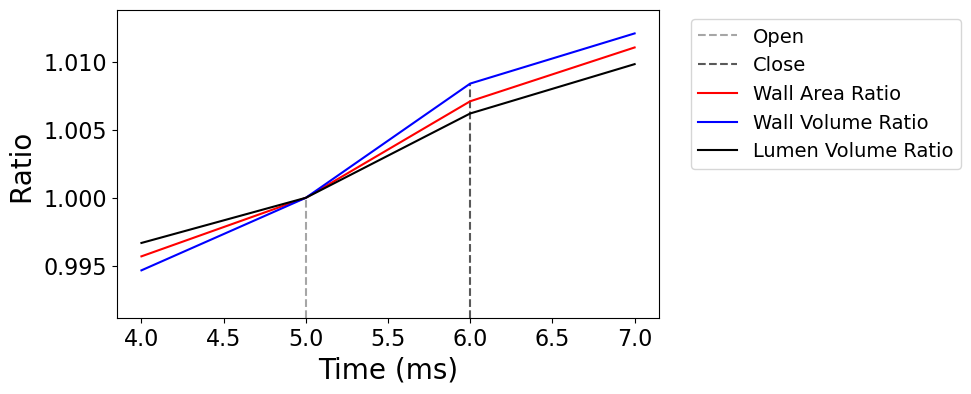
\includegraphics[width=0.75\textwidth]{NormalisedDataOriginalTime.png}
	\caption{Wall area, wall volume and lumen volume ratio, with original time data.}
\end{figure}


\begin{figure}[h!]
	\centering
	\includegraphics[width=0.75\textwidth]{NormalisedDataStandardisedTime.png}
	\caption{Wall area, wall volume and lumen volume ratio, with standardised time data.}
\end{figure}


\begin{figure}[h!]
	\centering
	\includegraphics[width=\textwidth]{RawDataOriginalTime.png}
	\caption{Raw data of wall area, wall volume and lumen volumes, with original time data.}
\end{figure}

\begin{figure}[h!]
	\centering
	\includegraphics[width=\textwidth]{RawDataStandardisedTime.png}
	\caption{Raw data of wall area, wall volume and lumen volume ratio, with standardised time data.}
\end{figure}



\end{document}
